In this section, we are going to solve the problem presented above with Comsol Multiphysics.

This is a Laplace equation and Comsol has already a nice setup for us. All we have to do is impose boundary conditions and generate the mesh. By default, Comsol sets zero flux boundary conditions so we just have to specify the Dirichlet conditions on the left and right sides. Once we have done this, we first use a mesh of type "normal". Figure \ref{mesh} shows what the "normal" mesh looks like for our geometry.

This mesh contains 316 triangles and 679 degrees of freedom. There are also 182 nodes.

\begin{figure}
\begin{center}
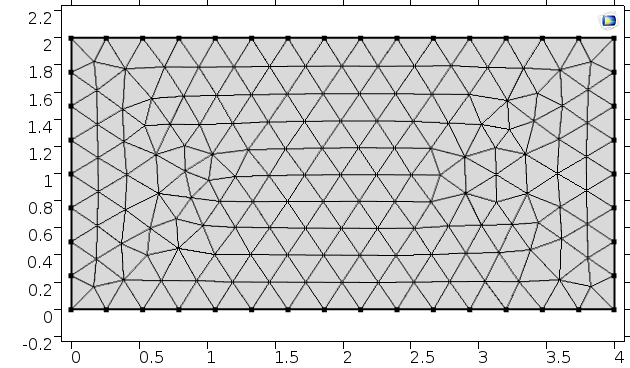
\includegraphics[scale=0.6]{laplaceMesh.png}
\caption{"Normal" mesh for the rectangular geometry}
\label{mesh}
\end{center}
\end{figure}

Figure \ref{rect} shows the solution for this choice of mesh. We can see that is it very similar to the one in section 1 which is a linear function between $x=0$ and $x=4$. We also used a probe to check the temperature at $(x,y)=(2,1)$.
$$T(2,1) = 450.0000000001594$$

That is very close to the analytic value and the error is only due to floating point computation.

We are now going to refine the mesh. We switch from "normal" to "fine". There are now 476 triangles and 1011 degrees of freedom, as well as 268 nodes.

We have another $T-value$ and:
$$T(2,1) = 450.000000000236$$

We can see that the two values are extremely close to each other and as we said, the small difference is due to floating point errors.

We finally restart all over again with a "normal" mesh. After having set all needed values, Comsol plots the solution given in figure \ref{rect}.


\begin{figure}
\begin{center}
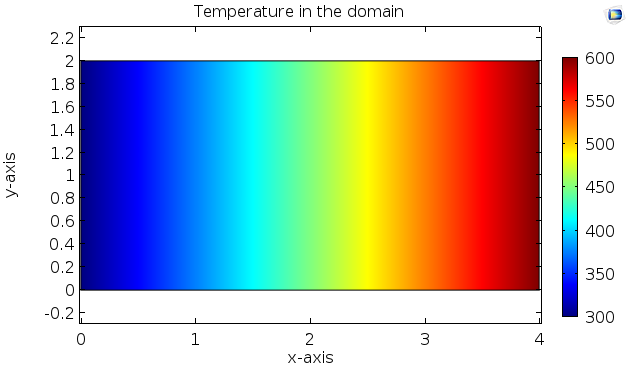
\includegraphics[scale=0.6]{laplaceRect.png}
\caption{Solution of the given problem with Comsol}
\label{rect}
\end{center}
\end{figure}